\section{Техническое задание}
\subsection{Основание для разработки}

Основанием для разработки является задание для курсовой работы по предмету   "<Проектирование и архитектура программных систем">.

\subsection{Цель и назначение разработки}

Основной задачей курсовой работы является разработка игры в жанре платформер на языке Python.

Основной целью данной работы является изучение проектирования и архитектуры программных систем на примере игры в жанре платформер .

Задачами данной разработки являются:
\begin{itemize}
\item создание основного геймплейного мира, включая уровни, платформы и препятствия;
\item реализация движения персонажа, включая прыжки, бег и способность взаимодействия с окружающей средой;
\item дизайн и внедрение графики, включая персонажей, фоны и анимации;
\item создание системы управления, такой как управление клавишами или сенсорным вводом;
\item разработка системы физики для реалистичного поведения персонажа и объектов в игре;
\item реализация механизмов столкновений;
\item создание игровой логики, включая счетчики очков, систему жизней и другие игровые механизмы;
\item интеграция звуковых эффектов и музыки для улучшения атмосферы игры;
\item тестирование и отладка игры для выявления и устранения ошибок и недоразумений.
\end{itemize}

\subsection{Требования пользователя к интерфейсу игры}

Игра должна включать в себя:
\begin{itemize}
    \item главное меню;
    \item основной игровой уровень, где игрок управляет персонажем и взаимодействует с платформами и препятствиями;
    \item механику сбора предметов;
    \item отслеживание и отображение собранных очков.
\end{itemize}

Композиция шаблона игры представлена на рисунке ~\ref{fig:1}.
\begin{figure}[ht]
	\centering
	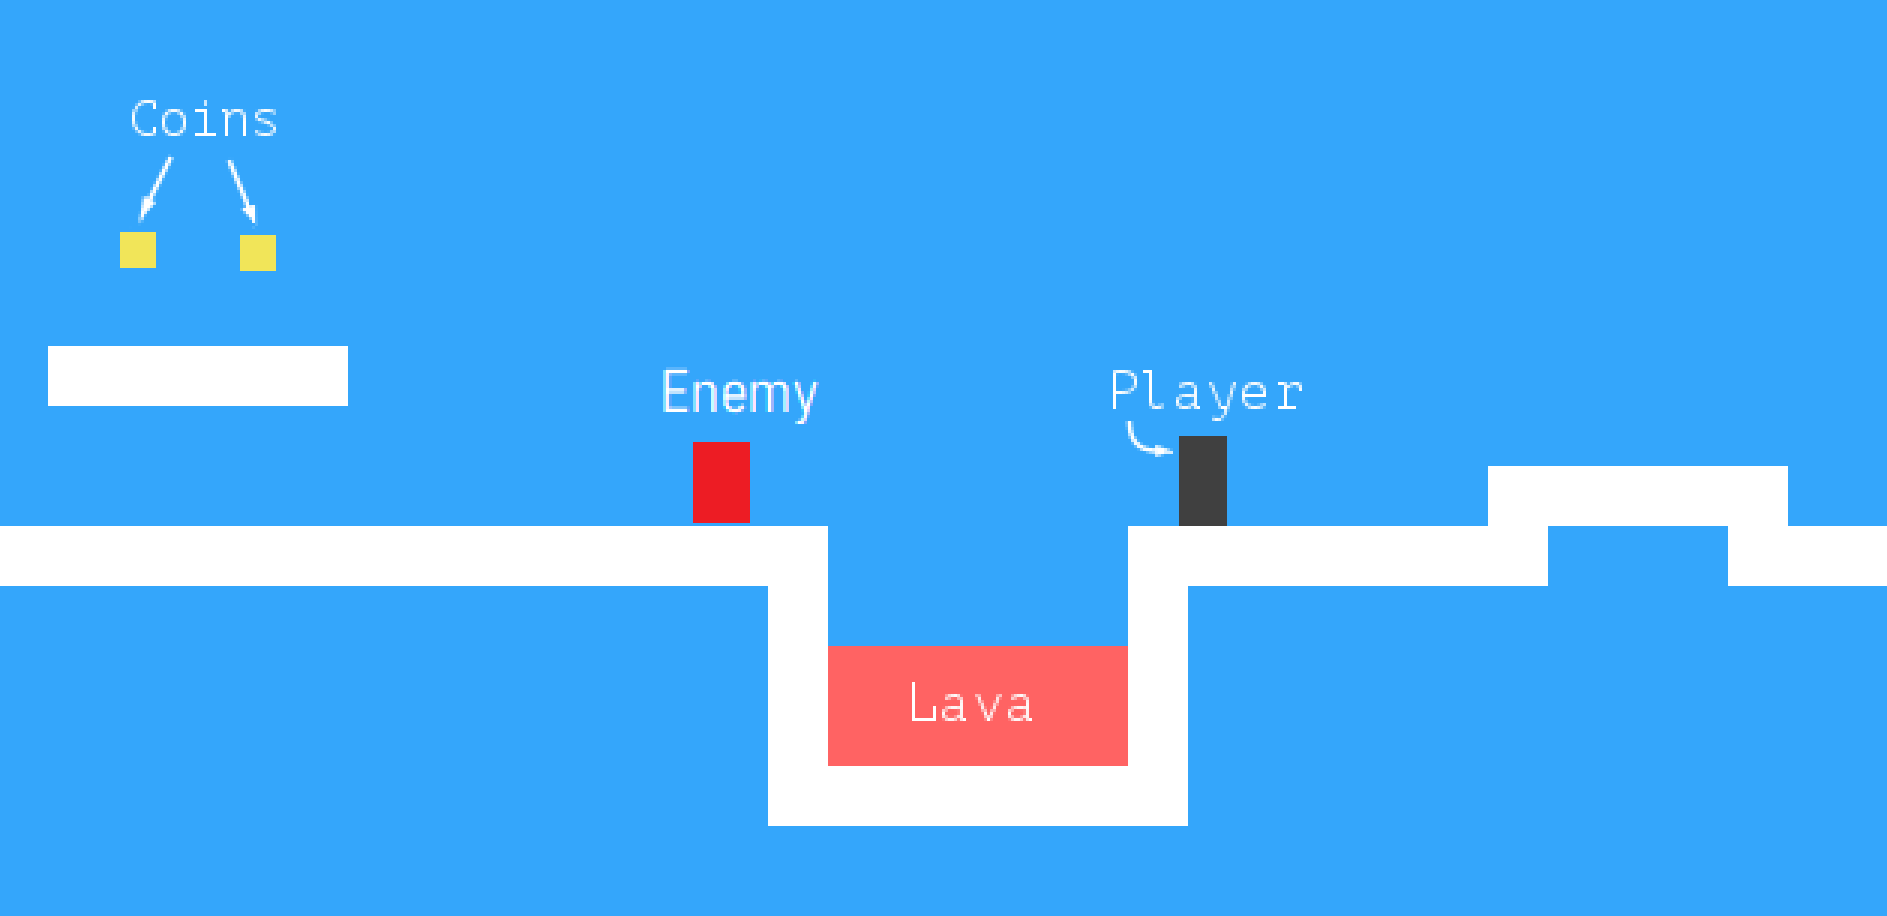
\includegraphics[width=1\linewidth]{images/Макет1}
	\caption{Композиция шаблона игры}
	\label{fig:1}
\end{figure}

%\begin{figure}[ht]
%\caption{Композиция шаблона сайта}
%\label{templ:image}
%\end{figure}
%\vspace{-\figureaboveskip} % двойной отступ не нужен (можно использовать, если раздел заканчивается картинкой)

\subsection{Моделирование вариантов использования}

Для разрабатываемой игры была реализована модель, которая обеспечивает наглядное представление вариантов использования игры.

Она помогает в физической разработке и детальном анализе взаимосвязей объектов. При построении диаграммы вариантов использования применяется унифицированный язык визуального моделирования UML.

Диаграмма вариантов описывает функциональное назначение разрабатываемой системы. То есть это то, что система будет непосредственно делать в процессе своего функционирования. Она является исходным концептуальным представлением системы в процессе ее проектирования и разработки. Проектируемая система представляется в виде ряда прецедентов, предоставляемых системой актерам или сущностям, которые взаимодействуют с системой. Актером или действующим лицом является сущность, взаимодействующая с системой извне (например, человек, техническое устройство). Прецедент служит для описания набора действий, которые система предоставляет актеру.

На основании анализа предметной области в программе должны быть реализованы следующие прецеденты:
\begin{enumerate}
\item Начать игру.
\item Управление персонажем.
\item Сбор предметов.
\item Столкновение с врагами.
\item Смерть и перезапуск уровня.
\item Завершение игры.
\end{enumerate}

\subsection{Требования к оформлению документации}

Разработка программной документации и программного изделия должна производиться согласно ГОСТ 19.102-77 и ГОСТ 34.601-90. Единая система программной документации.
